\documentclass[11pt,a4paper]{article}
\usepackage[T1]{fontenc}
\usepackage[utf8]{inputenc}
\usepackage{lmodern}
\usepackage{textcomp}
\usepackage[left=1.8cm,right=1.8cm,top=2.3cm,bottom=2.2cm,headheight=14pt,headsep=8pt]{geometry}
\usepackage{multicol}
\usepackage{xcolor}
\usepackage{fancyhdr}
\usepackage{graphicx}
\usepackage{array}
\usepackage{amsmath,amssymb}
\usepackage{setspace}
\usepackage{longtable}
\graphicspath{{../}}
\definecolor{ygreen}{RGB}{46,139,87}
\renewcommand{\normalsize}{\fontsize{10.9}{13.4}\selectfont}
\renewcommand{\familydefault}{\rmdefault}
\setlength{\parindent}{0pt}
\setlength{\columnsep}{0.8cm}
\setlength{\columnseprule}{0.4pt}
\setlength{\multicolsep}{3pt plus 1pt minus 1pt}
\renewcommand{\textsubscript}[1]{\ensuremath{_{\text{\fontsize{8}{8}\selectfont #1}}}}
\renewcommand{\textsuperscript}[1]{\ensuremath{^{\text{\fontsize{8}{8}\selectfont #1}}}}
\newcommand{\diqqat}[1]{\par\smallskip\noindent\textbf{Diqqat!} #1\par\medskip}
\newcommand{\javob}{\par\smallskip\noindent\textbf{Javob:} \rule[-2pt]{7.5cm}{0.4pt}\par\smallskip\noindent\textbf{Diqqat!} Javobingizni javoblar varaqasiga ko`chirib yozing.\par\medskip}
\pagestyle{fancy}
\fancyhf{}
\renewcommand{\headrulewidth}{0.4pt}
\fancyhead[L]{\textit{Milliy sertifikat 2026. Kimyo}}
\fancyhead[R]{19-variant}
\fancyfoot[L]{\fontsize{8}{9}\selectfont \textcopyright{} Colba maktabi, 2026}
\fancyfoot[C]{\thepage}
\fancypagestyle{first}{\fancyhf{}\renewcommand{\headrulewidth}{0pt}\fancyfoot[L]{\fontsize{8}{9}\selectfont \textcopyright{} Colba maktabi, 2026}\fancyfoot[C]{\thepage}}
\begin{document}
\normalsize
\thispagestyle{first}
\noindent\fcolorbox{ygreen}{white}{\parbox{\dimexpr\linewidth-2\fboxsep-2\fboxrule\relax}{%
\textbf{\fontsize{13}{15}\selectfont Nazorat testi}\ \textit{\fontsize{10}{12}\selectfont $\cdot$ Aralash test $\cdot$ 19-variant}\hfill
\begin{tabular}[t]{@{}r@{}}\textit{Milliy sertifikat 2026. Kimyo}\\ \textbf{\textit{\fontsize{8}{9}\selectfont Vaqt:}} \textit{\fontsize{10}{12}\selectfont 180 daqiqa}\end{tabular}}}
\par\medskip
\noindent\textit{Davriy jadvaldan foydalanish mumkin.}
\par\medskip
\begin{multicols}{2}
\noindent\textbf{1.} AgNO\textsubscript{3} eritmasi inert elektrodlar yordamida 4 A tok kuchi bilan 965 s elektroliz qilindi. Anodda ajralgan O\textsubscript{2} hajmi (l, n.sh.) \textbf{ni toping.}

\noindent A)~\textsl{0,448} \hfill B)~\textsl{0,224} \hfill C)~\textsl{0,112} \hfill D)~\textsl{0,009}\par
\vspace{4pt}
\noindent\textbf{2.} Xlor (\textit{Z} = 17) atomida nechta juftlashmagan elektron bor?

\noindent A)~\textsl{1} \hfill B)~\textsl{2} \hfill C)~\textsl{3} \hfill D)~\textsl{0}\par
\vspace{4pt}
\noindent\textbf{3.} Tabiiy elementning ikki izotopi: \textsuperscript{35}Cl (75\%) va \textsuperscript{37}Cl (25\%). Elementning o`rtacha nisbiy atom \textbf{massasini aniqlang.}

\noindent A)~\textsl{35,5} \hfill B)~\textsl{36} \hfill C)~\textsl{36,5} \hfill D)~\textsl{35}\par
\vspace{4pt}
\noindent\textbf{4.} Na\textsubscript{2}SO\textsubscript{4} eritmasiga 0,2 mol/l li BaCl\textsubscript{2} eritmasi oz-ozdan qo`shilganda hosil bo`lgan cho`kma massasining qo`shilgan hajmga bog`liqligi grafikda keltirilgan.
\begin{center}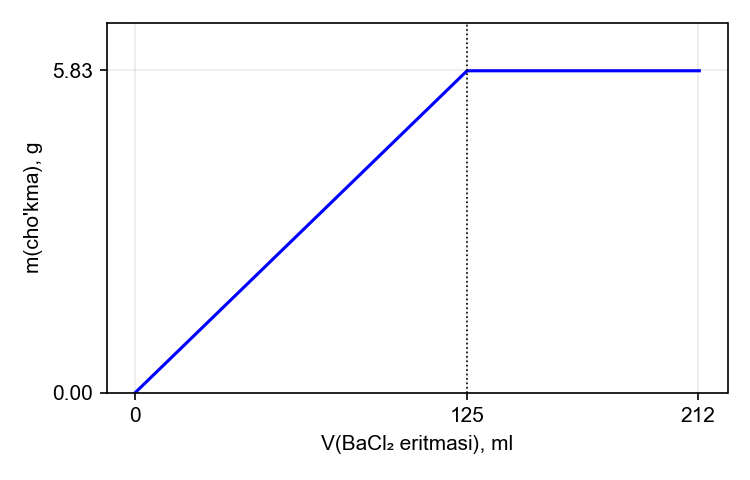
\includegraphics[width=0.86\linewidth]{rasmlar/gen/pp_v19_0.png}\end{center}
Grafikdagi cho`kma massasi 5,83 g da to`xtagan. Egri chiziq to`xtagan nuqtagacha qo`shilgan BaCl\textsubscript{2} ning \textbf{massasini (g) toping.}

\noindent A)~\textsl{5,83} \hfill B)~\textsl{3,55} \hfill C)~\textsl{10,4} \hfill D)~\textsl{5,2}\par
\vspace{4pt}
\noindent\textbf{5.} Rasmda radioaktiv yemirilish zanjiri berilgan (massa soni/zaryad; ``?'' -- oraliq yadrolar).
\begin{center}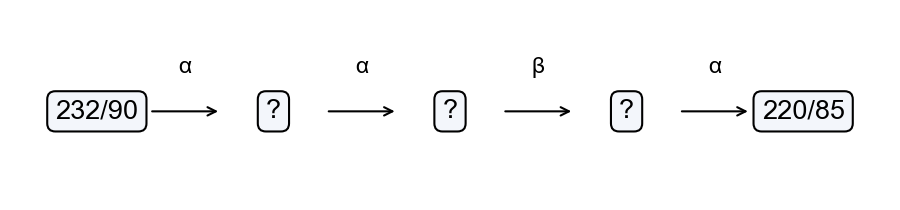
\includegraphics[width=0.86\linewidth]{rasmlar/gen/dc_549220.png}\end{center}
Oxirgi yadroning massa \textbf{sonini aniqlang.}

\noindent A)~\textsl{224} \hfill B)~\textsl{216} \hfill C)~\textsl{220} \hfill D)~\textsl{221}\par
\vspace{4pt}
\noindent\textbf{6.} Hajmi 5 l bo`lgan idishda A modda miqdori 30 s davomida 1,2 mol ga kamaydi. Reaksiyaning o`rtacha tezligini (mol/(l$\cdot$s)) \textbf{toping.}

\noindent A)~\textsl{0,04} \hfill B)~\textsl{0,24} \hfill C)~\textsl{0,008} \hfill D)~\textsl{0,2}\par
\vspace{4pt}
\noindent\textbf{7.} Quyidagi jadvalda CuSO\textsubscript{4} tuzining eritmalari keltirilgan:
\begin{center}
\renewcommand{\arraystretch}{1.15}
\begin{tabular}{|c|c|c|}\hline
\textbf{No.} & \textbf{m(eritma), g} & \textbf{$\omega$, \%} \\ \hline
I & 100 & 15 \\ \hline
II & 100 & 40 \\ \hline
\end{tabular}
\end{center}
Eritmalar aralashtirildi. Oxirgi eritmadagi tuzning massa \textbf{ulushini (\%) toping.}

\noindent A)~\textsl{55} \hfill B)~\textsl{24,75} \hfill C)~\textsl{13,75} \hfill D)~\textsl{27,5}\par
\vspace{4pt}
\noindent\textbf{8.} Jadvalda bog`lar hosil qiluvchi atomlarning elektrmanfiyliklari berilgan:
\begin{center}
\renewcommand{\arraystretch}{1.15}
\begin{tabular}{|c|c|c|}\hline
\textbf{Bog`} & \textbf{EM (1-atom)} & \textbf{EM (2-atom)} \\ \hline
Si--O & 1,8 & 3,5 \\ \hline
K--Br & 0,8 & 2,8 \\ \hline
H--F & 2,1 & 4 \\ \hline
H--N & 2,1 & 3 \\ \hline
\end{tabular}
\end{center}
Qaysi bog` eng qutbli (eng ko`p ionli xarakterga ega)?

\noindent A)~\textsl{Si--O} \hfill B)~\textsl{H--F} \hfill C)~\textsl{H--N} \hfill D)~\textsl{K--Br}\par
\vspace{4pt}
\noindent\textbf{9.} H\textsubscript{2} va CH\textsubscript{4} gazlari 3 : 4 hajmiy nisbatda aralashtirildi. Aralashmaning vodorodga nisbatan \textbf{zichligini aniqlang.}

\noindent A)~\textsl{5} \hfill B)~\textsl{10} \hfill C)~\textsl{6} \hfill D)~\textsl{4,5}\par
\vspace{4pt}
\noindent\textbf{10.} CH\textsubscript{4} gazining -23 \textdegree{}C va 2 atm bosimdagi \textbf{zichligini (g/l) aniqlang.} (R = 0,082 l$\cdot$atm/(mol$\cdot$K))

\noindent A)~\textsl{3,12} \hfill B)~\textsl{0,78} \hfill C)~\textsl{0,71} \hfill D)~\textsl{1,56}\par
\vspace{4pt}
\noindent\textbf{11.} CH\textsubscript{3}--CH=CH\textsubscript{2} molekulasida sp\textsuperscript{3} gibridlangan uglerod atomlari nechta?

\noindent A)~\textsl{2} \hfill B)~\textsl{3} \hfill C)~\textsl{1} \hfill D)~\textsl{4}\par
\vspace{4pt}
\noindent\textbf{12.} Faqat oksidlovchi bo`la oladigan \textbf{ionlarni aniqlang}: 1) Na\textsuperscript{+}; 2) Fe\textsuperscript{3+}; 3) S\textsuperscript{2$-$}; 4) I\textsuperscript{$-$}

\noindent A)~\textsl{2, 3} \hfill B)~\textsl{4} \hfill C)~\textsl{1} \hfill D)~\textsl{3}\par
\vspace{4pt}
\noindent\textbf{13.} H\textsubscript{3}PO\textsubscript{3} tarkibida P ning oksidlanish \textbf{darajasini aniqlang.}

\noindent A)~\textsl{+5} \hfill B)~\textsl{+3 va +5} \hfill C)~\textsl{$-$2} \hfill D)~\textsl{+3}\par
\vspace{4pt}
\noindent\textbf{14.} Reaksiya tenglamasi: SiO\textsubscript{2} + 2NaOH $\to$ Na\textsubscript{2}SiO\textsubscript{3} + H\textsubscript{2}O. Reaksiyaga tarkibida 20\% aralashma bo`lgan 20 g namuna (asosiy modda NaOH) kirishdi. Na\textsubscript{2}SiO\textsubscript{3} \textbf{massasini (g) hisoblang.}

\noindent A)~\textsl{97,6} \hfill B)~\textsl{24,4} \hfill C)~\textsl{48,8} \hfill D)~\textsl{12,2}\par
\vspace{4pt}
\noindent\textbf{15.} 2NaBr + Cl\textsubscript{2} $\to$ 2NaCl + Br\textsubscript{2} reaksiyasida 71 g Cl\textsubscript{2} ishtirok etdi. Br\textsubscript{2} \textbf{miqdorini (mol) toping.}

\noindent A)~\textsl{2} \hfill B)~\textsl{0,5} \hfill C)~\textsl{1,5} \hfill D)~\textsl{1}\par
\vspace{4pt}
\noindent\textbf{16.} Ishqoriy metallar haqida qaysi fikrlar to`g`ri? 1) KOH -- kuchli ishqor; 2) Natriy atomining tashqi qavatida 2 ta elektron bor; 3) Natriy kerosin ostida saqlanadi; 4) Natriy suv bilan reaksiyada H\textsubscript{2} va NaOH hosil qiladi

\noindent A)~\textsl{1, 2, 3} \hfill B)~\textsl{1, 3, 4} \hfill C)~\textsl{2, 3} \hfill D)~\textsl{1, 2, 4}\par
\vspace{4pt}
\noindent\textbf{17.} Mg\textsubscript{3}N\textsubscript{2} + 6H\textsubscript{2}O $\to$ 3Mg(OH)\textsubscript{2} + 2NH\textsubscript{3} jarayoni uchun 50 g Mg\textsubscript{3}N\textsubscript{2} olingan (unum 90\%). NH\textsubscript{3} \textbf{hajmini (l, n.sh.) aniqlang.}

\noindent A)~\textsl{5,6} \hfill B)~\textsl{20,16} \hfill C)~\textsl{40,32} \hfill D)~\textsl{10,08}\par
\vspace{4pt}
\noindent\textbf{18.} 11,2 g temir bir qismi xlor bilan, xuddi shuncha qismi xlorid kislota bilan reaksiyaga kirishdi. Hosil bo`lgan tuzlar massalari \textbf{farqini (g) aniqlang.}

\noindent A)~\textsl{32,5} \hfill B)~\textsl{7,1} \hfill C)~\textsl{25,4} \hfill D)~\textsl{14,2}\par
\vspace{4pt}
\noindent\textbf{19.} 0,05 mol Ca(HCO\textsubscript{3})\textsubscript{2} tutgan suv qaynatilganda hosil bo`lgan CaCO\textsubscript{3} cho`kma massasini (g)  \textbf{ni toping.}

\noindent A)~\textsl{5} \hfill B)~\textsl{10} \hfill C)~\textsl{2,5} \hfill D)~\textsl{7,5}\par
\vspace{4pt}
\noindent\textbf{20.} C\textsubscript{4}H\textsubscript{6} alkinlarning izomerlari soni nechta?

\noindent A)~\textsl{3} \hfill B)~\textsl{1} \hfill C)~\textsl{4} \hfill D)~\textsl{2}\par
\vspace{4pt}
\noindent\textbf{21.} CH\textsubscript{2}=CH--CH=CH\textsubscript{2} birikmaning sistematik nomi qaysi qatorda to`g`ri keltirilgan?

\noindent\begin{tabular}{@{}p{0.47\linewidth}@{}p{0.47\linewidth}@{}}
A)~\textsl{butadiyen-1,3} & B)~\textsl{butadiyen-1,2} \\
C)~\textsl{buten-1} & D)~\textsl{butin-1} \\
\end{tabular}\par
\vspace{4pt}
\noindent\textbf{22.} C\textsubscript{6}H\textsubscript{6} + HNO\textsubscript{3} $\to$ C\textsubscript{6}H\textsubscript{5}NO\textsubscript{2} + H\textsubscript{2}O reaksiyasida 156 g C\textsubscript{6}H\textsubscript{6} ishtirok etdi. HNO\textsubscript{3} \textbf{massasini (g) toping.}

\noindent A)~\textsl{252} \hfill B)~\textsl{126} \hfill C)~\textsl{63} \hfill D)~\textsl{189}\par
\vspace{4pt}
\noindent\textbf{23.} Spirt va fenollar haqida qaysi fikrlar to`g`ri? 1) Etilenglikol zaharsiz; 2) Etanol natriy bilan reaksiyaga kirishadi; 3) Glitserin Cu(OH)\textsubscript{2} bilan ko`k kompleks hosil qiladi; 4) Fenol Cu(OH)\textsubscript{2} ni eritib ko`k kompleks hosil qiladi

\noindent A)~\textsl{2, 3} \hfill B)~\textsl{4} \hfill C)~\textsl{3, 4} \hfill D)~\textsl{2, 4}\par
\vspace{4pt}
\noindent\textbf{24.} Aldegid va ketonlar haqida qaysi fikrlar to`g`ri? 1) Formalin --- formaldegidning 40\% li eritmasi; 2) Ketonlar kuchsiz oksidlovchilar bilan oksidlanmaydi; 3) Aldegidlar qaytarilganda ikkilamchi spirt hosil bo`ladi; 4) Aldegidlar "kumush ko`zgu" reaksiyasini beradi

\noindent A)~\textsl{2, 3} \hfill B)~\textsl{1, 2, 4} \hfill C)~\textsl{1, 3} \hfill D)~\textsl{1, 3, 4}\par
\vspace{4pt}
\noindent\textbf{25.} C\textsubscript{4}H\textsubscript{9}Cl galogenli hosilalarning izomerlari soni nechta?

\noindent A)~\textsl{4} \hfill B)~\textsl{5} \hfill C)~\textsl{3} \hfill D)~\textsl{6}\par
\vspace{4pt}
\noindent\textbf{26.} 12 g sirka kislota va 6,4 g metanol dan 80\% unum bilan murakkab efir olindi. Efir \textbf{massasini (g) toping.}

\noindent A)~\textsl{14,8} \hfill B)~\textsl{23,68} \hfill C)~\textsl{11,84} \hfill D)~\textsl{5,92}\par
\vspace{4pt}
\noindent\textbf{27.} Uglevodlar haqida qaysi fikrlar to`g`ri? 1) Glyukoza "kumush ko`zgu" reaksiyasini beradi; 2) Selluloza $\beta$-glyukoza qoldiqlaridan iborat; 3) Saxaroza Feling suyuqligini qaytaradi; 4) Maltoza gidrolizlanganda ikki molekula glyukoza hosil qiladi

\noindent A)~\textsl{1, 3} \hfill B)~\textsl{2, 4} \hfill C)~\textsl{1, 3, 4} \hfill D)~\textsl{1, 2, 4}\par
\vspace{4pt}
\noindent\textbf{28.} Reaksiya tenglamasi: NH\textsubscript{2}CH\textsubscript{2}COOH + NaOH $\to$ NH\textsubscript{2}CH\textsubscript{2}COONa + H\textsubscript{2}O. Reaksiyaga 37,5 g NH\textsubscript{2}CH\textsubscript{2}COOH kirishdi (unum 80\%). NH\textsubscript{2}CH\textsubscript{2}COONa \textbf{miqdorini (mol) hisoblang.}

\noindent A)~\textsl{0,5} \hfill B)~\textsl{0,8} \hfill C)~\textsl{0,4} \hfill D)~\textsl{0,2}\par
\vspace{4pt}
\noindent\textbf{29.} C\textsubscript{2}H\textsubscript{2} + HCl $\to$ C\textsubscript{2}H\textsubscript{3}Cl jarayoni uchun 3,65 g HCl olingan. C\textsubscript{2}H\textsubscript{3}Cl \textbf{massasini (g) aniqlang.}

\noindent A)~\textsl{12,5} \hfill B)~\textsl{3,12} \hfill C)~\textsl{6,25} \hfill D)~\textsl{9,38}\par
\vspace{4pt}
\noindent\textbf{30.} Rasmdagi tajribada qizdirilgan konsentrlangan HNO\textsubscript{3} parchalanadi. Ajralgan gaz qanday rangda?
\begin{center}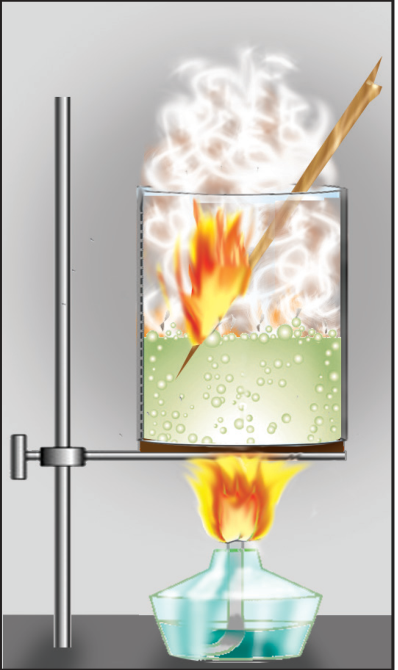
\includegraphics[width=0.86\linewidth]{rasmlar/darslik/d_hno3_yogoch.png}\end{center}

\noindent\begin{tabular}{@{}p{0.47\linewidth}@{}p{0.47\linewidth}@{}}
A)~\textsl{jigarrang (NO\textsubscript{2})} & B)~\textsl{yashil-sariq (Cl\textsubscript{2})} \\
C)~\textsl{rangsiz (N\textsubscript{2})} & D)~\textsl{ko`k (NO)} \\
\end{tabular}\par
\vspace{4pt}
\noindent\textbf{31.} Kimyo laboratoriyasida ishlash qoidalari haqida qaysi fikrlar to`g`ri? 1) Ortiqcha reaktiv idishga qaytariladi; 2) Konsentrlangan kislotani suvga ohista, aralashtirib quyiladi; 3) Kimyoviy moddalar hidini bevosita nafas olib aniqlash kerak; 4) Probirka qizdirilganda og`zi odamga qaratilmaydi

\noindent A)~\textsl{1, 2} \hfill B)~\textsl{1, 2, 3} \hfill C)~\textsl{2, 4} \hfill D)~\textsl{2, 3, 4}\par
\vspace{4pt}
\noindent\textbf{32.} Kimyoviy laboratoriyada ajratgich voronka nima uchun ishlatiladi?
\noindent A)~\textsl{probirkani qizdirish}\par
\noindent B)~\textsl{aralashmaydigan suyuqliklarni ajratish}\par
\noindent C)~\textsl{moddalarni namlikdan saqlash}\par
\noindent D)~\textsl{gaz (H\textsubscript{2}, CO\textsubscript{2}, H\textsubscript{2}S) olish   ---}\par
\vspace{4pt}
\end{multicols}
\medskip
\noindent\setlength{\fboxsep}{0pt}\fbox{\begin{tabular}{p{0.74\linewidth}|p{0.2\linewidth}}
\parbox[t]{0.72\linewidth}{\vspace{3pt}\textbf{Topshiriqlar (33--35) va javob variant (A--F)larini o`zaro to`g`ri moslashtiring.} KCl va NaBr dan iborat 22,9 g aralashma suvda eritilib, mo`l AgNO\textsubscript{3} eritmasi qo`shildi; hosil bo`lgan cho`kmalarning umumiy massasi 42,55 g.
\vspace{3pt}} & \parbox[t]{0.19\linewidth}{\vspace{3pt}A~\textsl{3,73}\\[3pt]
B~\textsl{45,7}\\[3pt]
C~\textsl{637,5}\\[3pt]
D~\textsl{7,45}\\[3pt]
E~\textsl{425}\\[3pt]
F~\textsl{22,85}}\\ \hline
\parbox[t]{0.72\linewidth}{\vspace{2pt}\textbf{33. Aralashmadagi KCl massasini (g) aniqlang.}\vspace{2pt}} & \\ \hline
\parbox[t]{0.72\linewidth}{\vspace{2pt}\textbf{34. Sarflangan 10\% li AgNO\textsubscript{3} eritmasining massasini (g) aniqlang (M(AgNO\textsubscript{3}) = 170 g/mol).}\vspace{2pt}} & \\ \hline
\parbox[t]{0.72\linewidth}{\vspace{2pt}\textbf{35. Eritmada hosil bo`lgan nitratlarning umumiy massasini (g) aniqlang.}\vspace{2pt}} & 
\end{tabular}}
\par\bigskip
\noindent\textbf{36.} KMnO\textsubscript{4} + KI + H\textsubscript{2}SO\textsubscript{4} $\to$ MnSO\textsubscript{4} + I\textsubscript{2} + K\textsubscript{2}SO\textsubscript{4} + H\textsubscript{2}O reaksiya tenglamasini elektron balans usulida tenglang va barcha koeffitsiyentlar \textbf{yig`indisini aniqlang.}
\javob
\noindent\textbf{37.} 1 l hajmli yopiq idishda 1 mol N\textsubscript{2}O\textsubscript{4} qizdirilganda N\textsubscript{2}O\textsubscript{4} $\rightleftarrows$ 2NO\textsubscript{2} muvozanati qaror topdi. Muvozanat aralashmasining vodorodga nisbatan zichligi 36,8 ga teng. Shu haroratdagi muvozanat \textbf{konstantasini (K, mol/l) hisoblang.}
\javob
\noindent\textbf{38.} Al, Fe va Cu dan iborat aralashma mo`l NaOH eritmasi bilan ta'sirlashganda 6,72 l (n.sh.) vodorod ajraldi; xuddi shunday massadagi aralashma mo`l HCl bilan ta'sirlashganda 8,96 l (n.sh.) vodorod ajraldi, erimay qolgan qoldiq (mis) massasi 3,2 g. Aralashmaning dastlabki \textbf{massasini (g) toping.}
\javob
\noindent\textbf{39.} Etilen va asetilendan iborat 2,24 l (n.sh.) aralashma bromli suvdan o`tkazilganda 24 g brom yutildi. Aralashmadagi asetilenning \textbf{hajmini (l, n.sh.) toping.}
\javob
\noindent\textbf{40.} Izopren dan olingan polimerning molyar massasi 6800 g/mol. Polimerlanish \textbf{darajasini aniqlang.}
\javob
\par\bigskip\begin{center}\textbf{\fontsize{13}{15}\selectfont YOZMA ISH}\end{center}
\noindent\textbf{41.} \textbf{Topshiriqni bajarish jarayonida barcha reaksiya tenglamalarini yozing. Miqdoriy va arifmetik hisoblashlarni (unga asos bo`lgan usul yoki formulani ko`rsatgan holda) uzviy ketma-ketlikda bajaring.}\par\smallskip
200 g 15\% li NaCl eritmasi inert elektrodlar yordamida 10 A tok kuchi bilan 3860 s elektroliz qilindi.\par
\noindent 1)Katodda va anodda ajralgan gazlarning hajmlarini (l, n.sh.) hisoblang.\par
\noindent 2)Elektrolizdan keyingi eritma massasini (g) aniqlang. Ajralgan gazlarning umumiy massasini (g) ham hisoblang.\par
\noindent 3)Elektrolizdan keyingi eritmada NaOH ning massa ulushini (\%) toping.\par
\noindent 4)Hosil bo`lgan NaOH ni to`liq neytrallash uchun 10\% li HCl eritmasidan necha gramm kerak? Hosil bo`lgan NaCl massasini (g) ham hisoblang.\par
\noindent 5)Anodda ajralgan xlor KI eritmasidan o`tkazilsa, ajralgan yod massasini (g) aniqlang. Anodda ajralgan xlorning massasini (g) ham toping.\par
\diqqat{Mazkur topshiriq kengaytirilgan javobni talab etib, uning yechilish usuli va shu usul asosidagi barcha hisoblash amallari javoblar varaqasida aks etishi lozim.}
\noindent\textbf{42.} Quyidagi o`zgarishlar zanjirida \textit{X}, \textit{Y}, \textit{Z} noma'lum organik moddalar:\par
\[\setlength{\fboxsep}{0pt}\text{C\textsubscript{6}H\textsubscript{12}O\textsubscript{6}}\xrightarrow{\text{bijg`ish}}\text{\textit{X}}\xrightarrow{\text{CuO, t\textdegree{}}}\text{\textit{Y}}\xrightarrow{\text{Ag\textsubscript{2}O, NH\textsubscript{3}}}\text{\textit{Z}}\xrightarrow{\text{Cl\textsubscript{2}, P}}\text{ClCH\textsubscript{2}COOH}\]
\noindent 1)C\textsubscript{6}H\textsubscript{12}O\textsubscript{6} $\to$ \textit{X} : reaksiya tenglamasini yozing; hosil bo`lgan moddani nomlang.\par
\noindent 2)\textit{X} $\to$ \textit{Y} : reaksiya tenglamasini yozing; hosil bo`lgan moddani nomlang.\par
\noindent 3)\textit{Y} $\to$ \textit{Z} : reaksiya tenglamasini yozing; hosil bo`lgan moddani nomlang.\par
\noindent 4)\textit{Z} $\to$ ClCH\textsubscript{2}COOH : reaksiya tenglamasini yozing; hosil bo`lgan moddani nomlang.\par
\diqqat{Mazkur topshiriq kengaytirilgan javobni talab etib, uning yechilish usuli va shu usul asosidagi barcha hisoblash amallari javoblar varaqasida aks etishi lozim.}
\noindent\textbf{43.} \textbf{Topshiriqni bajarish jarayonida barcha reaksiya tenglamalarini yozing. Miqdoriy va arifmetik hisoblashlarni (unga asos bo`lgan usul yoki formulani ko`rsatgan holda) uzviy ketma-ketlikda bajaring.}\par\smallskip
Alyuminiy, temir va misdan iborat 11,5 g aralashma bo`lakchalarga bo`lindi. Bir bo`lagi (butun aralashma) mo`l NaOH eritmasi bilan reaksiyaga kirishganda 3,36 l (n.sh.) vodorod ajraldi. Xuddi shunday tarkibli ikkinchi aralashma (11,5 g) mo`l xlorid kislota bilan reaksiyaga kirishganda 5,6 l (n.sh.) vodorod ajraldi (temir FeCl\textsubscript{2} ga o`tdi).\par
\noindent 1)Aralashmadagi har bir metallning massasini (g) va massa ulushini (\%) aniqlang (reaksiya tenglamalarini yozing).\par
\noindent 2)Xlorid kislota bilan reaksiyadan keyin qolgan qoldiq konsentrlangan HNO\textsubscript{3} da to`liq eritildi. Ajralgan gazning hajmini (l, n.sh.) aniqlang.\par
\noindent 3)Xlorid kislota bilan olingan eritmaga mo`l NaOH qo`shildi, hosil bo`lgan cho`kma ajratib olinib, havoda to`liq oksidlanguncha qoldirildi. Cho`kma massasini (g) toping.\par
\noindent 4)Mis nitrat eritmasi bug`latilib, quruq tuz qizdirilganda hosil bo`ladigan qattiq qoldiq massasini (g) va gazlar aralashmasining hajmini (l, n.sh.) aniqlang.\par
\noindent 5)Aralashmadagi alyuminiyni eritish uchun (2Al + 2NaOH + 6H\textsubscript{2}O $\to$ 2Na[Al(OH)\textsubscript{4}] + 3H\textsubscript{2}) 10\% li NaOH eritmasidan necha gramm kerak?\par
\diqqat{Mazkur topshiriq kengaytirilgan javobni talab etib, uning yechilish usuli va shu usul asosidagi barcha hisoblash amallari javoblar varaqasida aks etishi lozim.}
\newpage
\noindent\textbf{\fontsize{13}{15}\selectfont Nazorat testi}\ \textit{$\cdot$ 19-variant}\hfill \textbf{Javoblar kaliti}\par\smallskip\hrule\smallskip
\textit{Faqat o`qituvchi uchun.}\par\medskip
\noindent\textbf{1--32-savollar}\par\smallskip
\noindent\begin{tabular}{|c|c|c|c|c|c|c|c|c|c|c|c|c|c|c|c|}\hline
\textbf{1} & \textbf{2} & \textbf{3} & \textbf{4} & \textbf{5} & \textbf{6} & \textbf{7} & \textbf{8} & \textbf{9} & \textbf{10} & \textbf{11} & \textbf{12} & \textbf{13} & \textbf{14} & \textbf{15} & \textbf{16}\\\hline
\textsl{B} & \textsl{A} & \textsl{A} & \textsl{D} & \textsl{C} & \textsl{C} & \textsl{D} & \textsl{D} & \textsl{A} & \textsl{D} & \textsl{C} & \textsl{C} & \textsl{D} & \textsl{B} & \textsl{D} & \textsl{B}\\\hline
\textbf{17} & \textbf{18} & \textbf{19} & \textbf{20} & \textbf{21} & \textbf{22} & \textbf{23} & \textbf{24} & \textbf{25} & \textbf{26} & \textbf{27} & \textbf{28} & \textbf{29} & \textbf{30} & \textbf{31} & \textbf{32}\\\hline
\textsl{B} & \textsl{B} & \textsl{A} & \textsl{D} & \textsl{A} & \textsl{B} & \textsl{A} & \textsl{B} & \textsl{A} & \textsl{C} & \textsl{D} & \textsl{C} & \textsl{C} & \textsl{A} & \textsl{C} & \textsl{B}\\\hline
\end{tabular}\par\medskip
\noindent\textbf{33--35-savollar}\par\smallskip
\noindent\begin{tabular}{|c|c|c|}\hline \textbf{No} & \textbf{Javob} & \textbf{Qiymat}\\\hline
33 & \textsl{D} & 7,45\\\hline
34 & \textsl{E} & 425\\\hline
35 & \textsl{F} & 22,85\\\hline
\end{tabular}\par\medskip
\noindent\textbf{36--40-savollar}\par\smallskip
\noindent\begin{tabular}{|c|c|}\hline \textbf{No} & \textbf{To`g`ri javob}\\\hline
36 & 41\\\hline
37 & 0,333\\\hline
38 & 14,2\\\hline
39 & 1,12\\\hline
40 & 100\\\hline
\end{tabular}\par\medskip
\noindent\textbf{41--43-topshiriqlar: qisqa yechim}\par\smallskip
\noindent\textbf{41-topshiriq.}\par
\noindent 1) Q = 10$\cdot$3860 = 38600 C = 0,4 mol e\textsuperscript{$-$}; katod: 2H\textsubscript{2}O + 2e\textsuperscript{$-$} $\to$ H\textsubscript{2} + 2OH\textsuperscript{$-$}: n(H\textsubscript{2}) = 0,2 mol $\to$ \textbf{4,48 l}; anod: 2Cl\textsuperscript{$-$} $-$ 2e\textsuperscript{$-$} $\to$ Cl\textsubscript{2}: n(Cl\textsubscript{2}) = 0,2 mol $\to$ \textbf{4,48 l}\par
\noindent 2) 2NaCl + 2H\textsubscript{2}O $\to$ H\textsubscript{2} + Cl\textsubscript{2} + 2NaOH: m = 200 $-$ 0,4 (H\textsubscript{2}) $-$ 14,2 (Cl\textsubscript{2}) = \textbf{185,4 g}; m = 0,4 + 14,2 = \textbf{14,6 g}\par
\noindent 3) n(NaOH) = n(e\textsuperscript{$-$}) = 0,4 mol = 16 g $\to$ $\omega$ = \textbf{8,63\%}\par
\noindent 4) NaOH + HCl $\to$ NaCl + H\textsubscript{2}O: HCl 0,4 mol = 14,6 g; eritma 14,6/0,1 = \textbf{146 g}; m(NaCl) = 0,4$\cdot$58,5 = \textbf{23,4 g}\par
\noindent 5) Cl\textsubscript{2} + 2KI $\to$ 2KCl + I\textsubscript{2}: n(I\textsubscript{2}) = 0,2 mol $\to$ \textbf{50,8 g}; m(Cl\textsubscript{2}) = 0,2$\cdot$71 = \textbf{14,2 g}\par
\noindent Jami: M 15 + A 10 = 25 ball.\par
\noindent\textbf{42-topshiriq.}\par
\noindent 1) C\textsubscript{6}H\textsubscript{12}O\textsubscript{6} + bijg`ish $\to$ C\textsubscript{2}H\textsubscript{5}OH (etanol)\par
\noindent 2) C\textsubscript{2}H\textsubscript{5}OH + CuO, t\textdegree{} $\to$ CH\textsubscript{3}CHO (sirka aldegid (etanal))\par
\noindent 3) CH\textsubscript{3}CHO + Ag\textsubscript{2}O, NH\textsubscript{3} $\to$ CH\textsubscript{3}COOH (sirka kislota)\par
\noindent 4) CH\textsubscript{3}COOH + Cl\textsubscript{2}, P $\to$ ClCH\textsubscript{2}COOH (xlorsirka kislota)\par
\noindent Jami 25 ball.\par
\noindent\textbf{43-topshiriq.}\par
\noindent 1) NaOH bilan faqat Al: 2Al + 2NaOH + 6H\textsubscript{2}O $\to$ 2Na[Al(OH)\textsubscript{4}] + 3H\textsubscript{2}: n(Al) = 0,1 mol = 2,7 g; HCl bilan: Fe + 2HCl $\to$ FeCl\textsubscript{2} + H\textsubscript{2}: n(Fe) = 0,1 mol = 5,6 g; Cu = 3,2 g. $\omega$: Al 23,5\%, Fe 48,7\%, Cu 27,8\%\par
\noindent 2) Cu + 4HNO\textsubscript{3}(kons.) $\to$ Cu(NO\textsubscript{3})\textsubscript{2} + 2NO\textsubscript{2} + 2H\textsubscript{2}O: NO\textsubscript{2} 0,1 mol $\to$ \textbf{2,24 l}\par
\noindent 3) AlCl\textsubscript{3} + 4NaOH $\to$ Na[Al(OH)\textsubscript{4}] + 3NaCl (eriydi); FeCl\textsubscript{2} + 2NaOH $\to$ Fe(OH)\textsubscript{2}$\downarrow$ + 2NaCl; 4Fe(OH)\textsubscript{2} + O\textsubscript{2} + 2H\textsubscript{2}O $\to$ 4Fe(OH)\textsubscript{3}: \textbf{10,7 g}\par
\noindent 4) 2Cu(NO\textsubscript{3})\textsubscript{2} $\to$ 2CuO + 4NO\textsubscript{2} + O\textsubscript{2}: CuO 0,05 mol = \textbf{4 g}; NO\textsubscript{2} 0,1 + O\textsubscript{2} 0,025 = 0,125 mol $\to$ \textbf{2,8 l}\par
\noindent 5) n(NaOH) = n(Al) = 0,1 mol $\to$ 4 g; eritma 4/0,1 = \textbf{40 g}\par
\noindent Jami: M 15 + A 10 = 25 ball.\par
\par\bigskip\noindent\textbf{Mavzular taqsimoti}\par\smallskip
{\small\noindent\begin{longtable}{|c|p{7.2cm}|p{5.4cm}|c|}\hline \textbf{No} & \textbf{Mavzu} & \textbf{Tekshiriladigan ko`nikma} & \textbf{Ball}\\\hline
1 & 11-sinf 8-bob (Faradey qonunlari); Tirkashev \textit{V} bob & Hisoblash va masala yechish & 1\\\hline
2 & Tirkashev I bob; 8-sinf (elektron konfiguratsiya) & Bilim va tushunish & 1\\\hline
3 & 8-sinf (izotoplar) & Hisoblash va masala yechish & 1\\\hline
4 & Tirkashev \textit{V} bob (almashinish reaksiyalari, grafik) & Grafik tahlili & 1\\\hline
5 & 11-sinf (yadro reaksiyalari) & Rasm bo`yicha tahlil & 1\\\hline
6 & 8-sinf; Tirkashev VI bob & Hisoblash va masala yechish & 1\\\hline
7 & Tirkashev III bob (eritmalar, jadval) & Jadval tahlili & 1\\\hline
8 & 8-sinf (kimyoviy bog`lanish turlari, jadval) & Jadval tahlili & 1\\\hline
9 & 11-sinf (D) & Hisoblash va masala yechish & 1\\\hline
10 & 11-sinf (Mendeleyev--Klapeyron) & Hisoblash va masala yechish & 1\\\hline
11 & 10-sinf \S{}17 & Bilim va tushunish & 1\\\hline
12 & Tirkashev \textit{V} bob; 11-sinf 7-bob & Bilim va tushunish & 1\\\hline
13 & 8-sinf; Tirkashev \textit{V} bob (oksidlanish darajasi) & Bilim va tushunish & 1\\\hline
14 & 9-sinf; Tirkashev (P/C/Si, hisob) & Hisoblash va masala yechish & 1\\\hline
15 & 9-sinf; Tirkashev (galogenlar, hisob) & Hisoblash va masala yechish & 1\\\hline
16 & 9-sinf (ishqoriy metallar); Tashev & Bilim va tushunish & 1\\\hline
17 & 9-sinf; Tirkashev (IIA/IIIA metallar (Ca,Mg,Al), hisob) & Hisoblash va masala yechish & 1\\\hline
18 & 9-sinf; Tashev (temir) & Hisoblash va masala yechish & 1\\\hline
19 & 9-sinf \S{}24 (suv qattiqligi) & Hisoblash va masala yechish & 1\\\hline
20 & 10-sinf \S{}6, \S{}12, \S{}20, \S{}28 (izomeriya) & Bilim va tushunish & 1\\\hline
21 & 10-sinf (nomenklatura \S{}6, \S{}11, \S{}20, \S{}24--26) & Bilim va tushunish & 1\\\hline
22 & 10-sinf (aren, hisob) & Hisoblash va masala yechish & 1\\\hline
23 & 10-sinf (mavzuga oid paragraflar); Abdusamatov & Bilim va tushunish & 1\\\hline
24 & 10-sinf (mavzuga oid paragraflar); Abdusamatov & Bilim va tushunish & 1\\\hline
25 & 10-sinf \S{}6, \S{}12, \S{}20, \S{}28 (izomeriya) & Bilim va tushunish & 1\\\hline
26 & 10-sinf \S{}28 (efirlanish) & Hisoblash va masala yechish & 1\\\hline
27 & 10-sinf (mavzuga oid paragraflar); Abdusamatov & Bilim va tushunish & 1\\\hline
28 & 10-sinf (amin, hisob) & Hisoblash va masala yechish & 1\\\hline
29 & 10-sinf (pol, hisob) & Hisoblash va masala yechish & 1\\\hline
30 & 8-sinf (nitrat kislota, 28-rasm) & Rasm bo`yicha tahlil & 1\\\hline
31 & 7-sinf (xavfsizlik qoidalari); 10-sinf lab. & Bilim va tushunish & 1\\\hline
32 & 7-sinf (laboratoriya jihozlari) & Bilim va tushunish & 1\\\hline
33--35 & Aralash masala (moslashtirish) & Ko`p bosqichli hisob & 3\\\hline
36--40 & Qisqa javobli masalalar & Hisoblash & 5\\\hline
41--43 & Yozma ish & Usul va hisob (M, A) & 75\\\hline
\end{longtable}}
\end{document}
